\section{Introduction and Background}

    Cardiovascular diseases remain the leading cause of death (31.8\% of all deaths) in U.S., costing 320.1 billion each year \cite{mozaffarian_heart_2016}. One significant area that need improvements is heart valve replacement and repair procedures such as aortic valve repair using bioprosthetic heart valves (BHVs), where the mortality has not seen any major improvements since 1985 – the rate of survival after 10 years still remains only 29.7\%. Soft-tissue-derived exogenously cross-linked (EXL) biomaterials, which has only existed since the beginning of 1970s, is the dominant choice due to advantages in immunogenicity and flow dynamics over their mechanical counter parts 
    \cite{starr_artificial_2007}. However, our understanding of these materials and of the mechanisms of their failure is still incomplete. As such, current design and development is very empirical in nature – depending on trial and error, extrapolation from accelerated wear test and long periods of clinical testing. The need for better BHV design is further accelerated by the emergence of percutaneous devices such as the transcatherized aortic valve replacement (TAVR) \cite{bonow_accaha_2006}\cite{guidoin_marvel_2010}. TAVRs are an attractive alternative to open heart surgeries, especially for people at high surgical risk, as well as youth who may require multiple surgical replacements over their life-time. However, they are more often associated with peri-valvular regurgitation and is currently lacking in long term data pertaining to their durability \cite{guidoin_marvel_2010}. Existing TAVR data suggest only 2-year mortality rate of 33.9\% 
    \cite{kodali_two_2012} in general and 68\%
    for aortic valve stenosis \cite{makkar_transcatheter_2012}. Much of the existing challenges are associated with the necessary compact folded delivery system, which places additional constraints on their geometrical design and mechanical properties. It is clear that there is a strong need for better understanding in the mechanism associated with their failure and frameworks for predicting the long-term failure of these devices.
        
    

    
    
    
    
    
    
    Heart valves are complex multi-layered structures that prevent backflow by opening and closing depending on the direction of flow. There are four valves in the heart, consisting of two atrioventricular preventing backflow between the atriums and ventricles, the mitral (MV) and tricuspid valves (TV), and two semilunar preventing backflows from the aorta and to the vena cava, the aortic (AV) and pulmonary valves (PV) (Fig. \ref{fig:heartdiagram}). The coordinated movement of the four heart valves enables them to maintain unidirectional blood flow during the cardiac cycle. When healthy, heart valves are incredibly resilient, opening and closing approximately 3 - 4 billion times throughout an average life-span \cite{sacks_biomechanics_2009}. The pressure changes during the cardiac cycle expose the heart valves to constant changes in forces and hemodynamics. This physiological demand is especially harsh on the mitral and aortic valves, needing to withstand average pressures of 80mmHg for the aortic and 120mmHg for the mitral valve to sustain circulation throughout the rest of the body. The biomechanical properties of heart valves must be able to withstand and function efficiently in this complex mechanical environment. Thus, the heart valve leaflets develop and maintain an intricate, highly organized, and multi-scale connective tissue system that allows them to do so \cite{tao_heart_2012}. 

    
    More than five million people are diagnosed with heart valve disease in the United States (US) each year [5, 7], with approximately 95,000 annual valve replacement surgeries, and 20,000 deaths per year [8]. Although valve disease can occur in any of the four valves, diseases of the 
    

%-------------------	begin FIGURE 	-------------------%
\begin{figure}
\centering
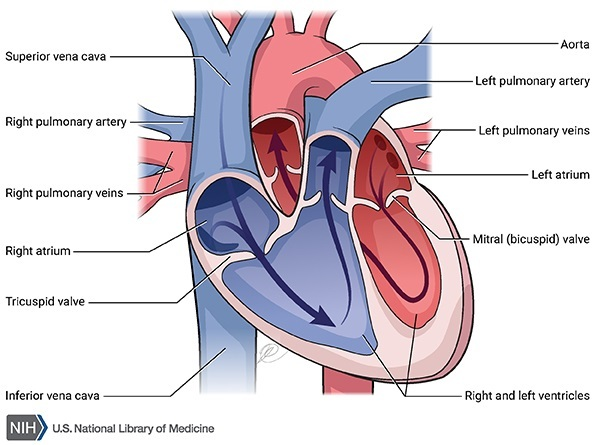
\includegraphics[width=5.0in]{Images/chapter1/heartdiagram.jpeg}
\caption{Artist rendition of the human heart depicting the location of the four heart valves and major vessels (obtained from U.S. National Library of Science website)}
\label{fig:heartdiagram}
\end{figure}
%-------------------	 end FIGURE 	-------------------%

